%% 4. 「技術研究報告」
\documentclass[technicalreport]{ieicej}
%\usepackage[dvips]{graphicx}
\usepackage[dvipdfmx]{graphicx,xcolor}
\usepackage[T1]{fontenc}
\usepackage{lmodern}
\usepackage{textcomp}
\usepackage{latexsym}
%\usepackage[fleqn]{amsmath}
\usepackage{amssymb}
\usepackage{subfigure}
\usepackage{url}

\jtitle{ LTE 環境における応答遅延特性の時系列モデリングによる分析}
\jsubtitle{}
\etitle{Analysis of delay characteristics of connection through LTE network\\ by time series analysis}
\esubtitle{}
\authorlist{%
 \authorentry[k-yamamt@ist.osaka-u.ac.jp]{山本 航平}{Kohei YAMAMOTO}{Osaka}
 \authorentry[wakamiya@ist.osaka-u.ac.jp]{若宮 直紀}{Naoki WAKAMIYA}{Osaka}
 \authorentry[ryo.nakano.xd@hitachi.com]{中野 亮}{Ryo NAKANO}{hitachi}
 \authorentry[ryosuke.fujiwara.mb@hitachi.com]{藤原 亮介}{Ryosuke FUJIWARA}{hitachi}
% \authorentry[メールアドレス]{和文著者名}{英文著者名}{所属ラベル}
}
\affiliate[Osaka]{大阪大学大学院情報科学研究科\\ 〒565-0871 大阪府吹田市山田丘 1-5}{Graduate School of Information Science and Technology, Osaka University\\ 1-5 Yamadaoka, Suita-shi, Osaka 565-0871, Japan}
\affiliate[hitachi]{株式会社日立製作所 研究開発グループ\\ 〒185-8601 東京都国分寺市東恋ヶ窪 1-280}{Research \& Development Group, Hitachi, Ltd.\\ 1-280 Higashikoigakubo, Kokubunji-shi, Tokyo  185-8601, Japan}
%\affiliate[所属ラベル]{和文勤務先\\ 連絡先住所}{英文勤務先\\ 英文連絡先住所}

\begin{document}

\newcommand{\argmin}{\mathop{\rm arg~min}\limits}
\def \vector#1{\mbox{\boldmath $#1$}}

\begin{jabstract}
%和文あらまし
産業用モニタリングシステムにおける運用管理コストの低減のため,迅速な障害検知・予測,ならびに原因の特定と対処法の提示が求められている.その実現にむけて,無線機器からサーバまでのLTE回線を含む通信路について,異なる曜日,時間帯において応答遅延の計測を行った.本稿では,応答遅延の変動特性や,曜日や時間帯に依存した傾向について,時系列モデリングおよびモデルパラメータにもとづくクラスタリングによって分析した.その結果,応答遅延の変動値の時系列モデリングにより応答遅延変動を捉えられること,また,モデルパラメータの主成分によってクラスタリングすることで曜日によらず 20 時台の計測データが同じクラスタに収容されるなど
応答遅延変動に共通性などの傾向が見られることを明らかにした.
\end{jabstract}
\begin{jkeyword}
%和文キーワード
Long Term Evolution,応答遅延,時系列モデリング,異常検知
\end{jkeyword}
\begin{eabstract}
%英文アブストラクト
Industrial monitoring systems are useful in remote monitoring, control, and diagnosis of equipments and facilities.
 For further reduction of operational and management cost, detection, prediction, and analysis of failures are strongly required in those systems.
 To achieve this, we measured response delays of connection from a wireless device to a cloud server through an LTE network in a variety of time of day and day of week.
 We first analyzed obtained data by time series analysis.
 Then we tried classification of them by clustering based on parameters of principal component analysis.
 As a result we revealed that we could grasp mid-term variation of response delay and there existed specific characteristics in accordance with time of day and day of week.
\end{eabstract}
\begin{ekeyword}
%英文キーワード
Long Term Evolution,response delay,time series analysis,anomaly detection
\end{ekeyword}
\maketitle

\section{はじめに}
近年,IoT (Internet of Things) 技術の発展とともに産業用モニタリングシステム\cite{lima2012embedded}が普及している.
これは,工場などの産業施設に設置された機器から直接,あるいは配置したカメラやセンサーなどの IoT デバイスを通じて,機器の稼働状態に関する情報をリアルタイムで収集し,キャリア回線を通じてクラウドサーバに送信,データ処理を行い,運用管理担当者に提示するものである.
作業員の巡回による工場内の機器の点検業務を自動化できるため,人員コストの軽減,目視確認より生じる人的ミスの低減,リアルタイムなデータの利活用などの効果が期待できる.
一方で,長期間の運用のなかで機器に具備された IoT デバイスの故障,工場内ネットワークの通信の途絶,クラウドサーバへの通信の遅延などの障害は避けられない.
このような障害が発生した場合には工場内の機器の稼働状況を把握することが困難となり,工場の稼働停止や業務の遅れなどが引き起こされ大きな損失をもたらす可能性がある.

障害発生時には迅速な復旧作業が求められるが,障害の原因や内容,規模はさまざまである.
しかしながら,現状ではシステムから得られる情報を用いてこれらの障害を適切かつ迅速に区別することが困難であるため,障害発生時には運用管理担当者が直接現場に行き障害の原因や内容,規模を確認する必要があり,多大な運用管理コストが発生している.
そのため,モニタリングシステムによる運用管理コストの低減のためには,直接また間接的に取得できる情報にもとづいて,障害発生を迅速に検知また予測するとともに,障害の原因を特定し,加えてその対処法を示すことが求められている.

我々の研究グループでは機器間で測定される受信電波強度の時間変化にもとづいて空間的な電波伝搬特性の変動を推定することにより工場内での無線通信の異常を検知する手法を提案している\cite{prev}.
本稿では工場内で機器稼働情報を収集する無線機器からクラウドサーバまでの通信路で発生する異常の検知手法の確立を目的とし,その第一段階としてさまざまな曜日,時間帯で応答遅延を計測し,応答遅延変動の分析を行う.
キャリア回線としては産業用モニタリングシステムに広く用いられている LTE(Long Term Evolution)回線を用いる.
LTE 回線の特性評価に関する研究としては,応答遅延の他の無線回線との比較評価\cite{striegel2014lte}\cite{garcia2015delay}や TCP パケットの振る舞いに関する調査\cite{huang2013depth},人の混雑状況と遅延分布に関する分析\cite{distribution}などが行われている.
本稿では,産業用モニタリングシステムを想定した4週間にわたる継続的な計測実験を行い,得られた応答遅延を時系列モデリングやクラスタリングによって分析し,その特性を見いだす.

第 2 章では本稿で実施した計測実験の設定について述べる.
第 3 章では時系列モデルによる回帰について述べる.
第 4 章では回帰結果を用いたクラスタリングによる分析について述べる.
第 5 章では全体のまとめと今後の課題について述べる.
\section{計測実験の設定}
本稿では図 \ref{exp} に示す構成で計測実験を行った.
モニタリングシステムにおける無線端末としては LTE モジュールとして Quectel 社製 EC21-J を搭載した Raspberry Pi を用いた.
また,LTE 回線としては IIJ モバイル社のサービスタイプ D 定額プランライト(いちねん プリペイド)を用いた.
IIJ モバイル社は他の通信事業者から通信回線を借り受け,サービスを提供している MVNO(Mobile Virtual Network Operator)であり,サービスタイプ D では NTT ドコモ社の回線を使用している.
月あたり通信量が 3GB を超過すると通信速度が 256kbps に制限されるが,本実験中には速度制限は課されなかった.

クラウドサーバとしては実験やシステム開発のために契約した一台の AWS サーバを用い,大阪大学敷地内の研究室に設置した Raspberry Pi から ping を用いて応答遅延を計測した.
自動的に計測データを取得できるよう,Raspberry Pi 上で動作する Raspbian において,15 秒毎に時刻を取得した後に ping (パケットサイズ 60 バイト, ICMP ECHO メッセージ,パケット数 1)で応答遅延を計測するスクリプトを実行した.
計測時刻,ping の出力をログデータとして取り出し,分析を行った.

通信時間帯が応答遅延に与える影響を調べるため,3 時,7 時,12 時,17 時,20 時のそれぞれ 1 時間において計測を行った.
それぞれの時間帯ごとに得られた計測値を区間データと呼ぶ.
計測は 2020 年 2 月 29 日(土)から 3 月 27 日(金)までの 4 週間に渡って行った.
したがって,区間数は 140,総計測数は 33600 となるが,一部の区間で Raspberry Pi の動作不良等による計測データの欠損が発生したため,それらの区間を除く 122 区間の計 29280 の計測値について分析を行った.

\begin{figure}[tb]
\centering
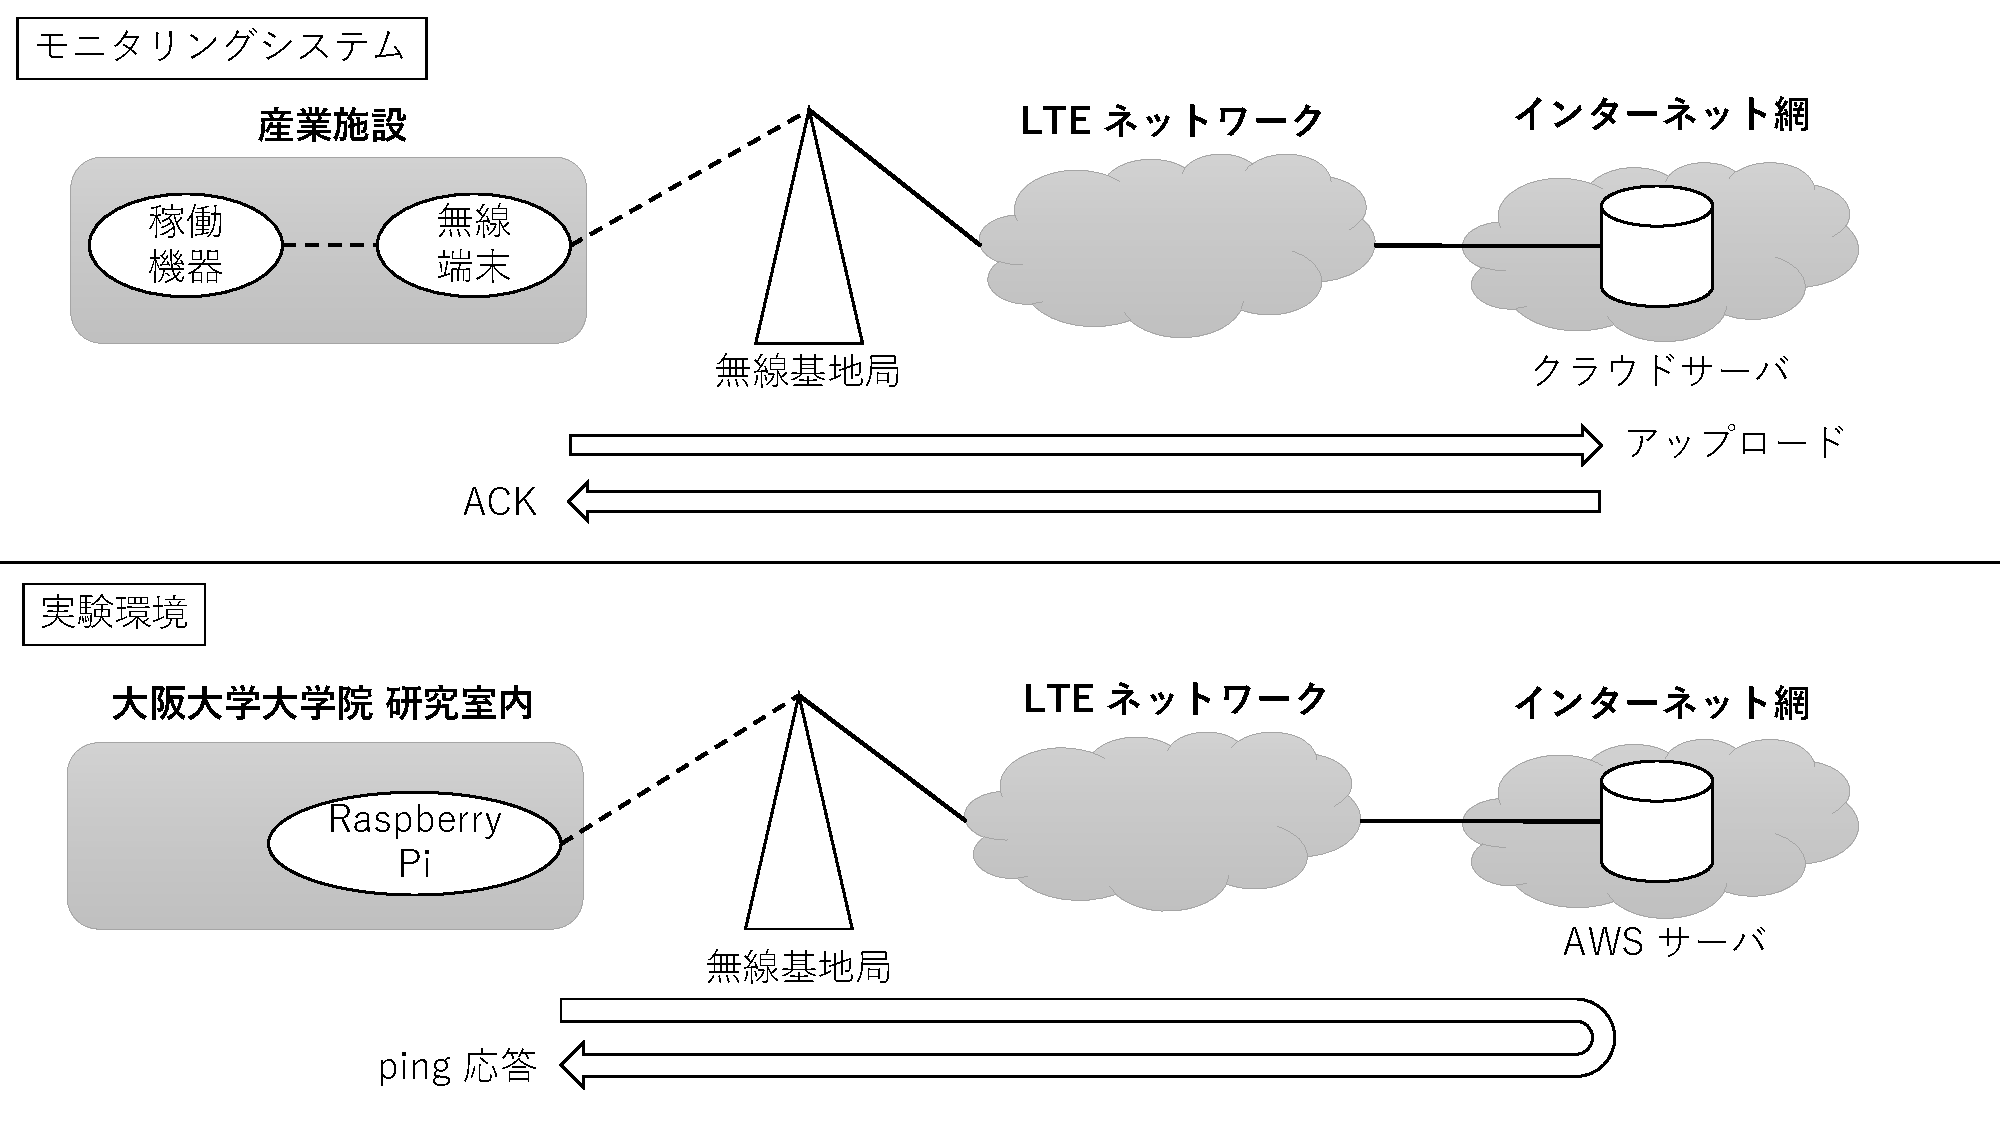
\includegraphics[width=7.5cm]{./figure/experiment.pdf}
\caption{モニタリングシステムと実験環境の対応}
\label{exp}
\end{figure}

\section{時系列モデルによる回帰}
本研究では,時系列モデルとして式 (\ref{garch1}) $\sim$ 式 (\ref{garch2}) で表される ARMA-GARCH(Autoregressive Moving Average - Generalized Autoregressive Conditional Heteroscedasticity)モデル\cite{lamoureux1990persistence}を用いる.
\begin{eqnarray}
y_t = \sum_{i=1}^p a_i x_{t-i} + \sum_{i=1}^q b_i (x_{t-i} - \widehat{y}_{t-i}) + c + \varepsilon_{t} 
\label{garch1}
\end{eqnarray}
\begin{eqnarray}
\widehat{y}_t = \sum_{i=1}^p a_i x_{t-i} + \sum_{i=1}^q b_i (x_{t-i} - \widehat{y}_{t-i}) + c
\end{eqnarray}
\begin{eqnarray}
\displaystyle h_{t} = \omega + \sum_{i=1}^{r}\alpha_i(x_{t-i} - \widehat{y}_{t-i})^2 + \sum_{i=1}^{s}\beta_ih_{t-i}
\label{garch2}
\end{eqnarray}
\begin{table}[b]
\centering
\caption{最適次数と共通次数での対数尤度の比較}
\label{more-param}
\begin{tabular}{|l|c|c|}
\hline
&最適次数での対数尤度&共通次数での対数尤度\\
\hline
実測値データ&-969.8327&-971.9196\\
\hline
変動値データ&-924.6495&-922.7543\\
\hline
\end{tabular}
\end{table}
ここで,$\varepsilon_t$ は平均 0,分散 $h_t$ の独立同一分布に従うノイズ項であり,分散 $h_t$ は式 (\ref{garch2}) で定められる.また, $\widehat{y}_i = x_i$ $(i = 1,2,\ldots,q)$ である.
時系列モデルによる回帰では,適切な次数 $p,q,r,s$ のもとで推定値 $y_t$ の時系列が実測値 $x_t$ の時系列を最も精度良くモデル化できるパラメータ $a_i,b_i,c,\omega,\alpha_i,$および $\beta_i$ を算出する.
$x_t$ $(1\leq t\leq N,N=240)$ は1時間の計測区間のそれぞれにおける計測時刻順の実測値である.
したがって,時刻 $t$ における推定値 $y_t$ は,定数項 $c$ と過去の $p$ 時点前までの実測値と $q$ 時点前までの誤差のそれぞれの重み付き和とノイズ項によって表される.
また,式 (\ref{garch2}) において,時刻 $t$ におけるノイズ項が従う正規分布の分散 $h_t$ は,定数項 $\omega$ と過去の $r$ 時点前までの誤差と $s$ 時点前までのノイズ項が従う正規分布の分散のそれぞれの重み付き和によって表される.

次数 $(p,q,r,s)$ は対象とする時系列データに応じて適切に定める必要がある.
最適な次数は区間データごとに異なるが,クラスタリングによる分類,分析のために共通の次数を用いることとする.
次数 $0\leq p\leq2,0\leq q\leq 2,r=1$,および $0\leq s\leq 1$ のそれぞれの組み合わせに対してAIC(赤池情報量規準)\cite{bozdogan1987model}\cite{burnham2004multimodel}を求めたところ,最大次数である $(p,q,r,s)=(2,2,1,1)$ が最適な計測区間が存在することから,これを共通の次数として用いることとした.
なお,式 (\ref{garch1}) における $p,q$ は次元数を抑えるために 2 まで,また,式 (\ref{garch2}) における $r,s$ は一般的に十分な性能が得られる 1 までとした\cite{hansen2005forecast}.
また,実測値$ x_t$ の代わりに実測値の差分である変動値の系列 $\{\Delta x_t | x_t - x_{t-1} \}$ に対する時系列解析についても検討を行ったところ,同様に $(p,q,r,s)=(2,2,1,1)$ を用いることとなった.
なお,AIC による最適次数よりも大きい次数を適用することの回帰精度への影響を検証するため,実測値における最適次数が $(0,1,1,0) $である区間データに対して次数 $(2,2,1,1)$ を適用した際の対数尤度の比較したところ,その変化量は約 0.2\% であった(表 \ref{more-param}).

\begin{figure}[tb]
\begin{center}
\subfigure[3/2(月)7:00-8:00]{
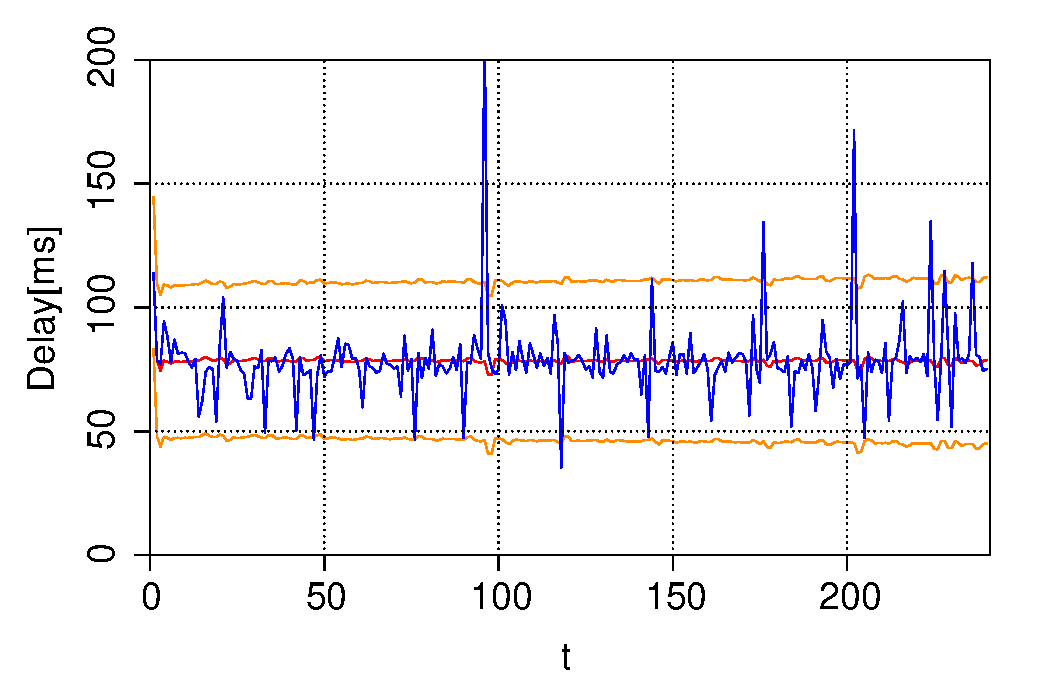
\includegraphics[height = 0.4\hsize,width=0.45\hsize]{./figure/0302_07-plot.pdf}
}~
\subfigure[3/9(月)7:00-8:00]{
\hspace*{-0.5cm}
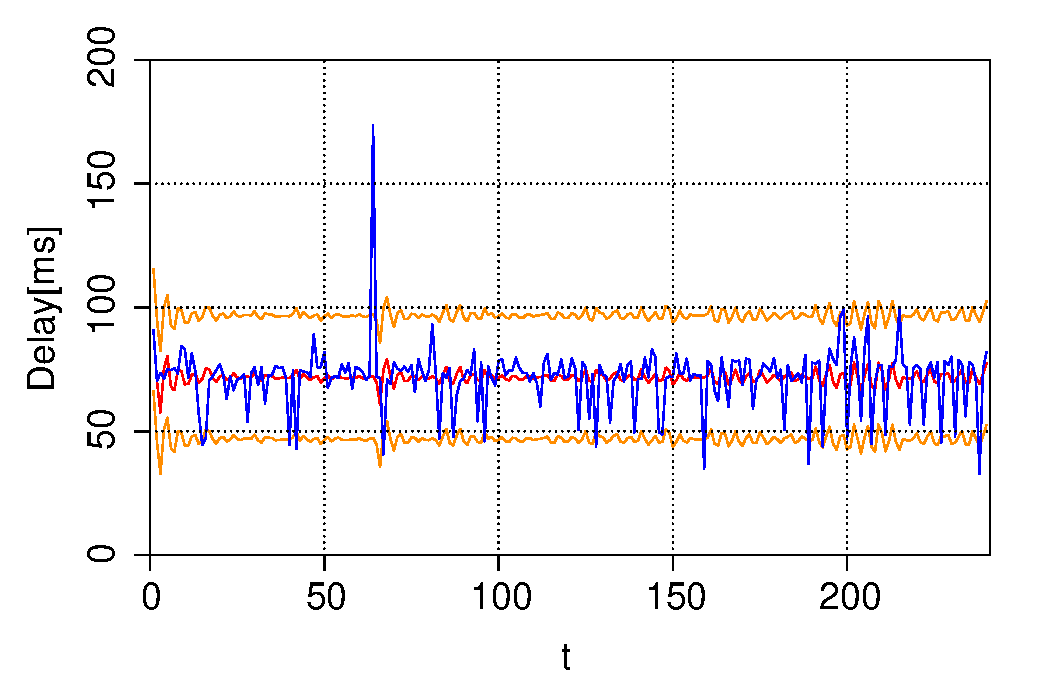
\includegraphics[height = 0.4\hsize,width=0.45\hsize]{./figure/0309_07-plot.pdf}
}~
\subfigure{
\hspace*{-0.5cm}
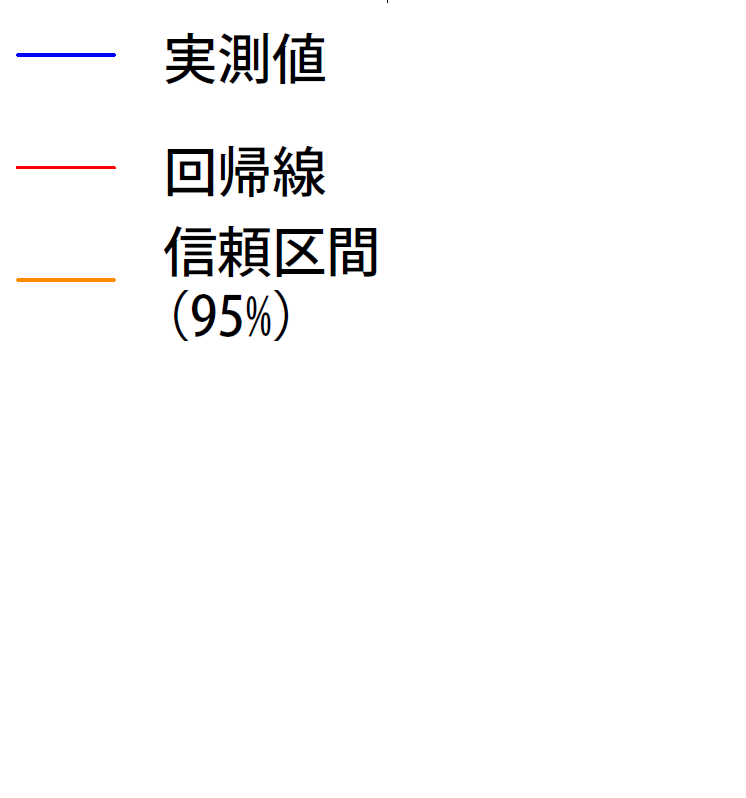
\includegraphics[height = 0.2\hsize,width=0.2\hsize]{./figure/norm-legend.png}
}
\caption{応答遅延の実測値の回帰結果}
\label{norm-reg}
\end{center}
\end{figure}

\begin{table}[tb]
\centering
\caption{応答遅延の実測値のモデルパラメータ}
\label{norm-param}
\begin{tabular}{|c|c|c|}
\hline
&(a) 3/2(月)7:00-8:00&(b) 3/9(月)7:00-8:00\\
\hline
$a_1$&-0.06019205&-0.19235040\\
\hline
$a_2$&-0.11082113&-0.76329719\\
\hline
$b_1$&0.01858739&0.17460199\\
\hline
$b_2$&0.06935663&0.65314854\\
\hline
$c$&91.83487587&140.40728113\\
\hline
$\omega$&0.20250175&8.66125582\\
\hline
$\alpha_1$&0.00000001&0.00000001\\
\hline
$\beta_1$&0.99999999&0.94672654\\
\hline
\end{tabular}
\end{table}

図 \ref{norm-reg} に異なる週の月曜日の 7:00~8:00 において得られた実測値に対する回帰結果を,表 \ref{norm-param} にこれらの時系列データに対するモデルのパラメータをそれぞれ示す.
図中の青線は実測値 $x_t$ を表している.
また,赤線は回帰によって得られたパラメータを式 (\ref{garch1}) の右辺第 4 項を除いて適用して求めた推測値 $y_t$ を,橙色の線は右辺第4項を加味した 95\% 信頼区間をそれぞれ示している.
図より,推定値は実測値の細かな変動を捉えられていないことがわかる.
特に最小応答遅延時間と考えられる約 40 ms の小さな応答遅延や単発的に発生する 100 ms 以上の大きな応答遅延を推定できていない.
これらの回帰結果における推定値と実測値の平均二乗誤差はそれぞれ 245.396,159.0008,ノイズ項を加味した対数尤度はそれぞれ -1000.131,-948.7874 であった.
また一方で,ずれはあるものの推定値は実測値の平均的な振る舞いにおおよそ追従しており,時系列モデリングにより中期的な応答遅延変動の傾向を捉えられている.
また,表 \ref{norm-param} より,同一曜日,時間帯であってもパラメータには差があることがわかる.
特に,3 月 9 日の方が $a_1$ と $a_2$ の絶対値が大きく,過去の実測値とより強い相関があることを示している.
したがって,3 月 9 日の応答遅延変動は実測値の大きさが時間的に持続しており,3 月 2 日と異なる振る舞いを示していると考えられる.

\begin{figure}[tb]
\begin{center}
\subfigure[3/2(月)7:00-8:00]{
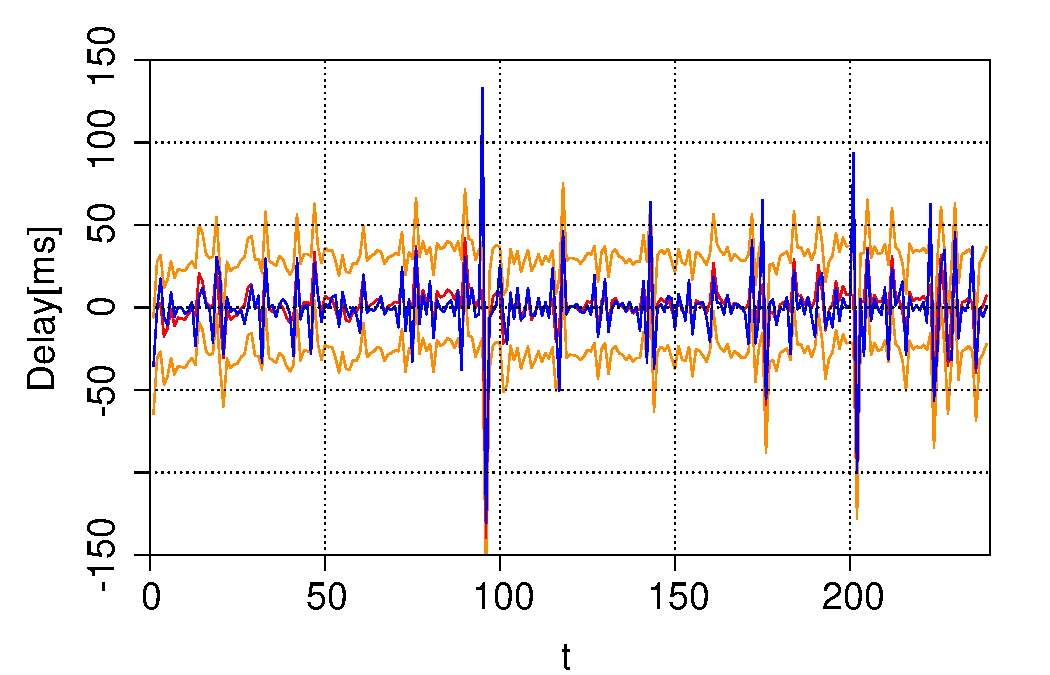
\includegraphics[height = 0.4\hsize,width=0.45\hsize]{./figure/0302_07-plot-diff.pdf}
}~
\subfigure[3/9(月)7:00-8:00]{
\hspace*{-0.5cm}
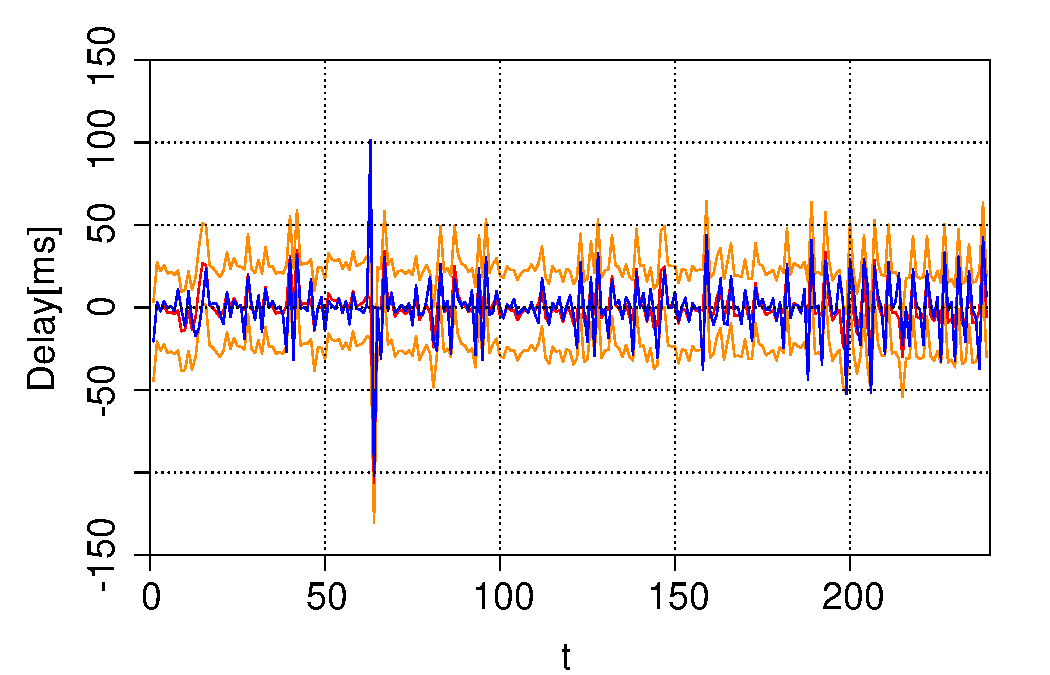
\includegraphics[height = 0.4\hsize,width=0.45\hsize]{./figure/0309_07-plot-diff.pdf}
}~
\subfigure{
\hspace*{-0.5cm}
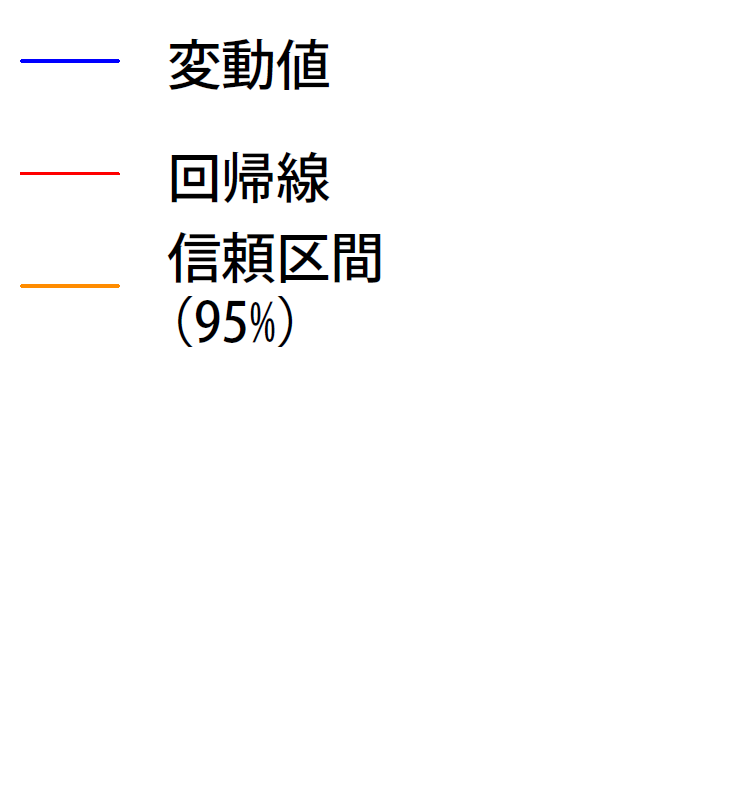
\includegraphics[height = 0.2\hsize,width=0.2\hsize]{./figure/diff-legend.png}
}
\caption{応答遅延の変動値の回帰結果}
\label{diff-reg}
\end{center}
\end{figure}

\begin{table}[tb]
\centering
\caption{応答遅延の変動値のモデルパラメータ}
\label{diff-param}
\begin{tabular}{|c|c|c|}
\hline
&(a) 3/2(月)7:00-8:00&(b) 3/9(月)7:00-8:00\\
\hline
$a_1$&-0.22605053&-0.67683663\\
\hline
$a_2$&-0.06377989&-0.01662159\\
\hline
$b_1$&-0.90702979&-0.42991003\\
\hline
$b_2$&-0.17145273&-0.67824234\\
\hline
$c$&-0.07518171&-0.08615516\\
\hline
$\omega$&166.42677036&8.33052597\\
\hline
$\alpha_1$&0.00000001&0.00000001\\
\hline
$\beta_1$&0.25766368&0.94593359\\
\hline
\end{tabular}
\end{table}

一方,同じ区間データにおける変動値にもとづく回帰結果とパラメータをそれぞれ図 \ref{diff-reg},表 \ref{diff-param} に示す.
図より,推定値は変動値の時間変化におおよそ追従しており,これらの回帰結果における推定値と変動値の平均二乗誤差はそれぞれ 223.2082,149.9259,ノイズ項を加味した対数尤度はそれぞれ -985.3953,-937.789 であったことからも,実測値の場合と比べてよく回帰できていると言える.
またスパイク状の突発的な応答遅延の増加は直前の応答遅延と無関係に発生するため,瞬時的には推定値との差が大きくなるが,その直後の応答遅延の減少は推定できている.
一方,表 \ref{diff-param} に示されるとおり,実測値の場合に比べて顕著ではないもののモデルパラメータに違いが見られた.
特に $\omega$ には 20 倍の違いがあり,これは 3 月 2 日の方が変動値の変化のばらつきが大きいことを示している.
したがって,3 月 2 日の応答遅延変動は変動値の大きく,変動値が異なる振る舞いを示していることがわかる.

以上より,時系列モデリングにもとづいて異常検知を行う際には,回帰の良さから実測値の変化量である変動値を用いるのがよく,例えば,あらかじめ算出したパラメータによって推定される変動値と実測によって得られる変動値を比較し,その差が大きい状態が継続した場合に異常とみなす,
あるいは,リアルタイムに逐次的な回帰を行い,パラメータが大きく変化した場合に異常とみなすなどの手法が有効であると考えられる.

\section{クラスタリングにもとづく分析}
 ARMA-GARCH モデルを実測値または変動値の区間データに適用して得られるパラメータ $\vector{W} = [a_1, a_2, b_1, b_2, c, \omega, \alpha_1, \beta_1]$ をもとにクラスタリングを行い,曜日や時間帯の異なる計測結果の類似性や傾向を分析する.
 まず,各パラメータの分布が異なるため,平均 0,標準偏差 1 となるように標準化を行う.
具体的には,区間データ $j$ のパラメータを $\vector{W_j} = [w_{j1},...,w_{j8}]$,パラメータ $w_{ji}$ の区間データ間の平均を $\mu_i$,標準偏差を $\sigma_i$ とすると,区間データ $j$ の標準化後のパラメータ $\vector{W_j^\prime} = [w_{j1}^\prime,...,w_{j8}^\prime]$ は次式で得られる.
$$w_{ji}^\prime = \frac{w_{ji} - \mu_i}{\sigma_i}$$
以降では簡単のため,このようにして得た標準化後のパラメータをそれぞれ実測値パラメータ,変動値パラメータと呼ぶ. 

次に,実測値パラメータ,変動値パラメータを主成分分析\cite{jolliffe2016principal}することで次元を削減する.
これは,実測値パラメータ,変動値パラメータの次元が高いことによって,一部のパラメータの細かな差異が重視されて本来同一の傾向がある区間データが異なるクラスタに収容されるなどの問題を抑制するためである.
実測値,変動値それぞれのパラメータ $\vector{W^\prime}$ に対して主成分分析を行った結果の累積寄与率を表 \ref{comp-load} に示す.
実測値パラメータ,変動値パラメータのいずれにおいてもおよそ $80\%$ の累積寄与率が得られている第三主成分までを用いてクラスタリングを行うこととする.
また,各主成分の主成分負荷量を表 \ref{comp-param} に示す.
表より,パラメータ $a_1,b_1,b_2$ が実測値,変動値のいずれに対しても第一主成分に大きく寄与していることがわかる.
従って,実測値,変動値の時間変化においては,一時点前の実測値や変動値,また,二時点前までの誤差の関わり方が区間データを特徴付けていると考えられる.

\begin{table}[tb]
\begin{center}
\caption{累積寄与率}
\label{comp-load}
\begin{tabular}{|l|l|l|l|l|}
\hline
&第一主成分&第二主成分&第三主成分&第四主成分\\
\hline
実測値パラメータ&0.449& 0.681& 0.863& 0.968\\
\hline
変動値パラメータ&0.367& 0.653& 0.794& 0.905\\
\hline
\end{tabular}
\end{center}
\end{table}

\begin{table}[tb]
\begin{center}
\caption{主成分負荷量}
\label{comp-param}
\subfigure[実測値パラメータ]{
\begin{tabular}{|l|l|l|l|}
\hline
&第一&第二&第三\\
&主成分&主成分&主成分\\
\hline
$c$&0.515&0.133& \\
$a_1$&-0.418&&-0.490\\
$a_2$&-0.404&-0.166&0.492\\
$b_1$&0.424&&0.475\\
$b_2$&0.391&0.157&-0.516\\
$\omega$&-0.119&0.569&0.101\\
$\alpha_1$&-0.142&0.432&\\
$\beta_1$&0.175&-0.643&-0.111\\
\hline
\end{tabular}
}~
\subfigure[変動値パラメータ]{
\begin{tabular}{|l|l|l|l|}
\hline
&第一&第二&第三\\
&主成分&主成分&主成分\\
\hline
$c$&&&0.721\\
$a_1$&0.571&&\\
$a_2$&&-0.190&-0.067\\
$b_1$&-0.571&&\\
$b_2$&0.574&&\\
$\omega$&&0.553&-0.127\\
$\alpha_1$&&0.499&\\
$\beta_1$&&-0.629&\\
\hline
\end{tabular}
}
\end{center}
\end{table}

\begin{figure}[tb]
\vspace*{-0.8cm}
\begin{center}
\subfigure[実測値パラメータの主成分]{
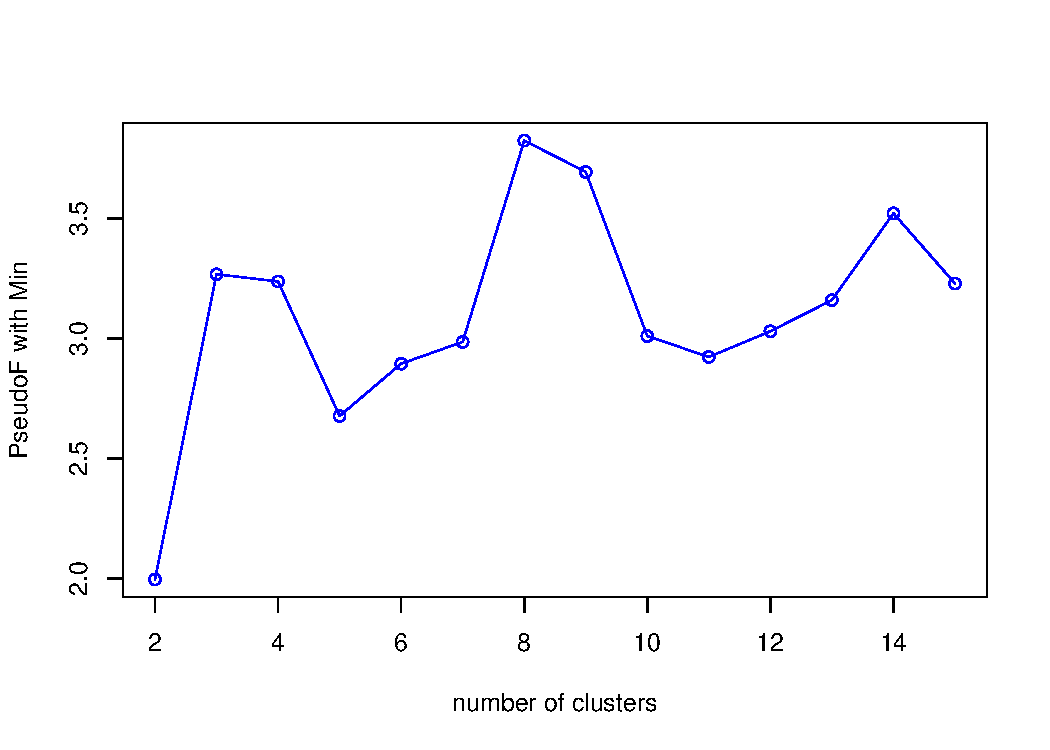
\includegraphics[height=0.43\hsize,width=0.5\hsize]{./figure/norm_comp-PseudoFwithMin.pdf}
}~
\subfigure[変動値パラメータの主成分]{
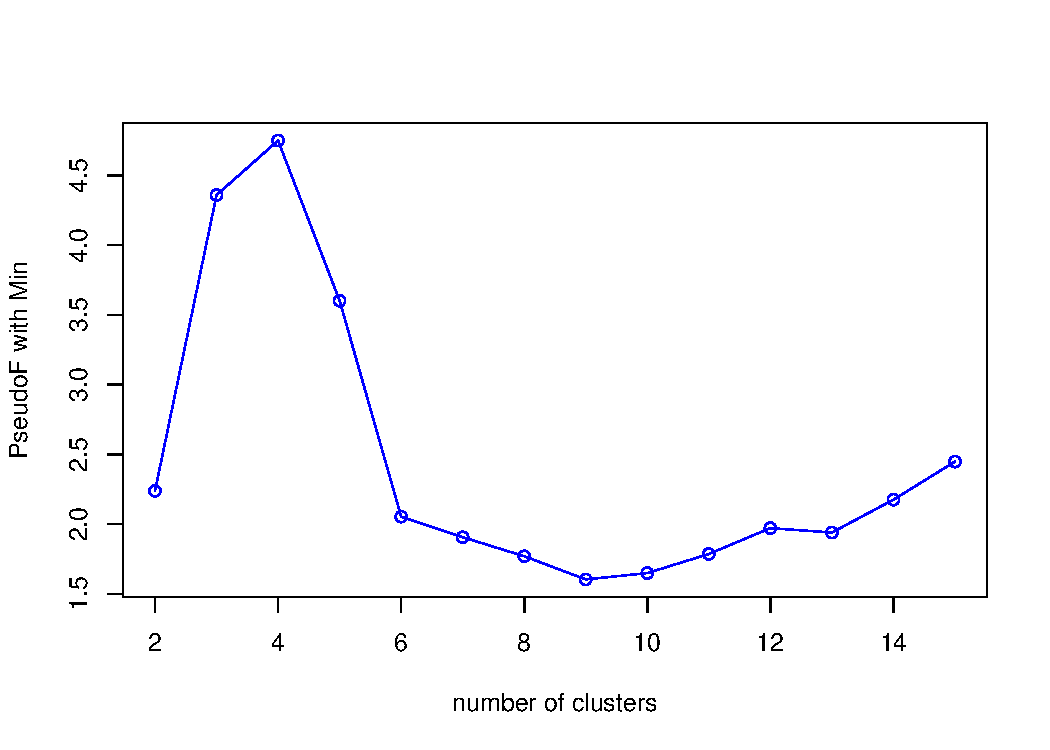
\includegraphics[height=0.43\hsize,width=0.5\hsize]{./figure/diff_comp-PseudoFwithMin.pdf}
}
\caption{クラスタ数と Pseudo F with Min の関係}
\label{PseudoFwithMinPlot}
\end{center}
\end{figure}
クラスタリングには,距離関数としてユークリッド距離を,また,階層クラスタリング手法の一つであるウォード法\cite{murtagh2014ward}を用いる.なお,距離関数としてはキャンベラ距離,マンハッタン距離,クラスタリング手法としては k-means 法,最近隣法,重心法についても試したが上記の組み合わせが最もデータの分離性能が高かった.
ウォード法では,融合後のクラスタ内分散と融合前の二つのクラスタ内分散の差が最小となるクラスタの組み合わせを順次融合する.

クラスタリングによってデータを分析するためには適切なクラスタ数を定める必要がある.
本研究においては,クラスタリング指標の一つである Pseudo F(Calinski Harabasz基準)\cite{liu2010understanding}に我々の研究グループで改良を加えた Pseudo F with Min\cite{kanajiri} を用いて定量的に最適なクラスタ数を決定する.
Pseudo F はクラスタ間分散のクラスタ内分散に対する比として与えられ,クラスタ間の離散性が高く,クラスタ内の凝集性が高い場合に値が大きくなる.
しかしながら,Pseudo F におけるクラスタ間分散は,全要素の代表点に対するクラスタの代表点のばらつきで定義されており,クラスタ同士の距離を反映していない.
そのため,Pseudo F の評価値が高くても,クラスタ間が密である可能性がある.
そこで,クラスタ間分散ではなく最近傍クラスタとの距離を用いるのがPseudo F with Min であり,式 (\ref{PseudoFwithMin}) で評価値が得られる.
\begin{equation}
\frac{\sum^k_{i=1} n_{i}\hspace{0.1cm} \min \{ dist(\vector{m_{i}},\vector{m_j})^2,j \neq i \}}{1 + \sum^k_{i=1} \sum_{\vector{x} \in C_i - \{\vector{m_i}\}} dist(\vector{x},\vector{m_{i}})^2}
\label{PseudoFwithMin}
\end{equation}
ここで,$k$ はクラスタ数,$C_1,\ldots,C_k$ はクラスタ集合を表し,要素数 $n_i=|C_i|$ である.
また,$\vector{m_i}$ はクラスタ $i$ の代表点であるメドイドである\cite{mouratidis2005medoid}.
$dist(\vector{x},\vector{y})$ は要素 $\vector{x}$ と $\vector{y}$ のユークリッド距離である.
実測値パラメータおよび変動値パラメータの主成分についてクラスタ数を変化させて Pseudo F with Min を求めた結果を図 \ref{PseudoFwithMinPlot} に示す.図より,実測値パラメータの場合にはクラスタ数 8 で,変動値パラメータの場合にはクラスタ数 4 でそれぞれ Pseudo F with Min が最大になることがわかる.

このもとでクラスタリングを行った結果を図 \ref{norm} と図 \ref{diff} に示す.
横軸に示すそれぞれのクラスタについて,各時間帯の区間データ数とその占める割合をそれぞれ図 (a)と図 (c) に示し,また各曜日の区間データ数とその区間データが占める割合をそれぞれ図 (b) と図 (d) に積み上げグラフで示している.
また,図 (e) では,横軸を曜日ごと,さらに時間帯で区切り,各クラスタに属する区間データの割合を積み上げグラフで示している.
各曜日,時間帯の区間データ数を上部に示す.

\begin{figure}[tb]
\begin{center}
\subfigure[時間帯での分類(区間データ数)]{
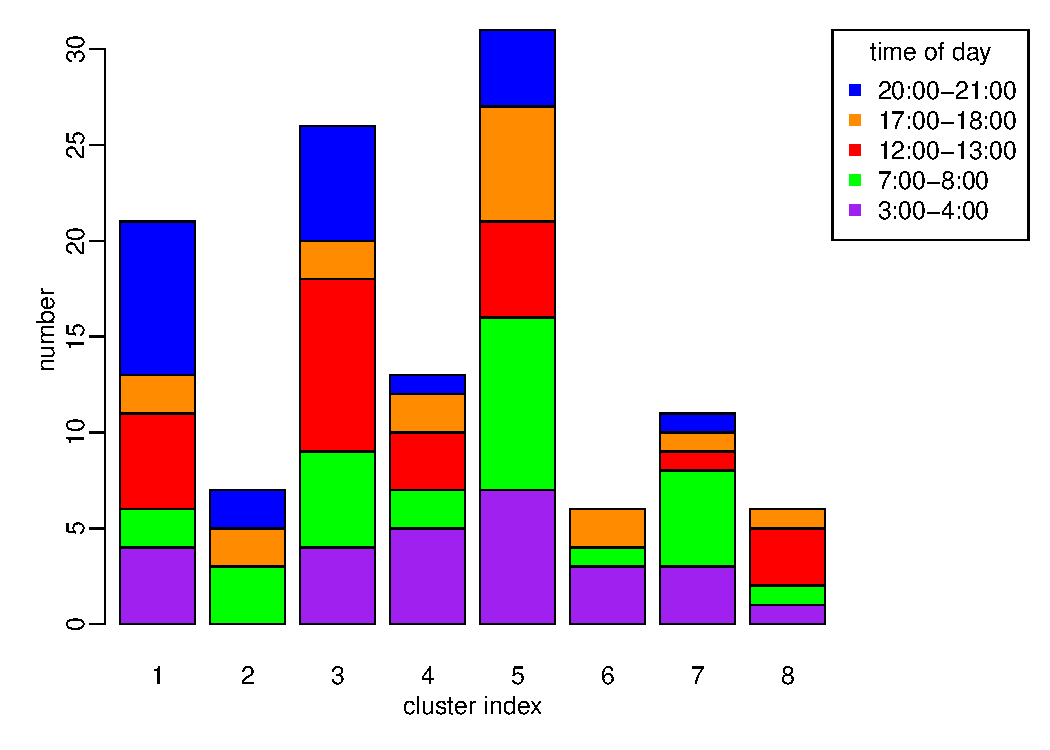
\includegraphics[height=0.42\hsize,width=0.53\hsize]{./figure/num-norm_comp-eucl-ward-8-timezone.pdf}
}~
\subfigure[曜日での分類(区間データ数)]{
\hspace*{-0.6cm}
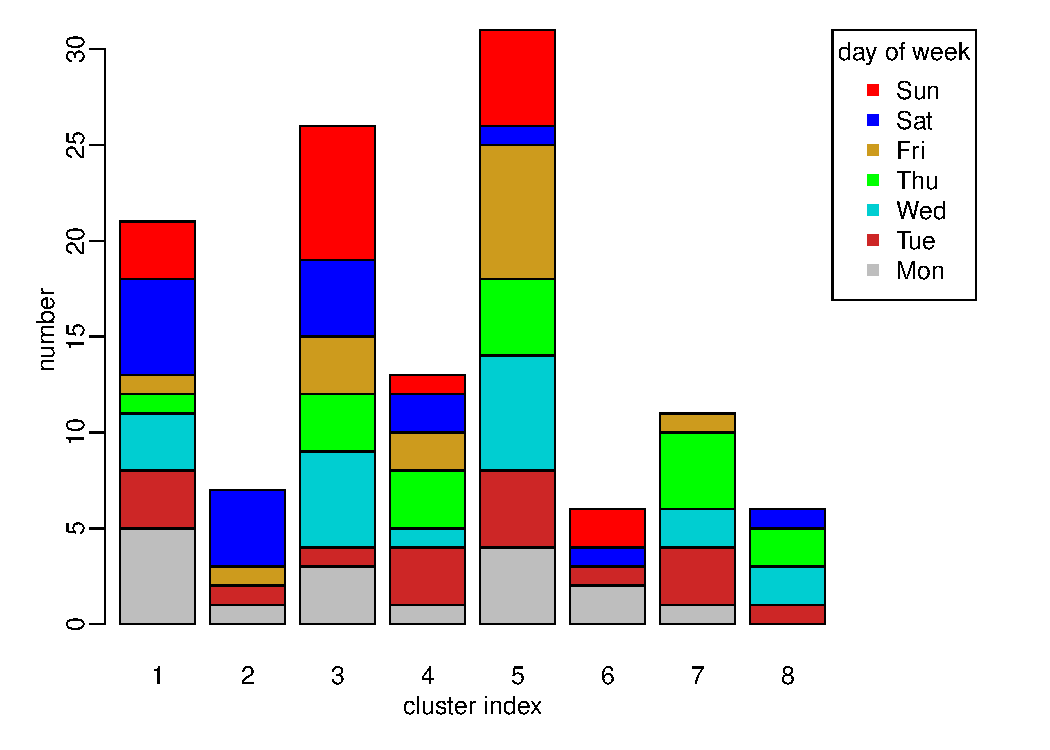
\includegraphics[height=0.42\hsize,width=0.53\hsize]{./figure/num-norm_comp-eucl-ward-8-day.pdf}
}\\
\subfigure[時間帯での分類(割合)]{
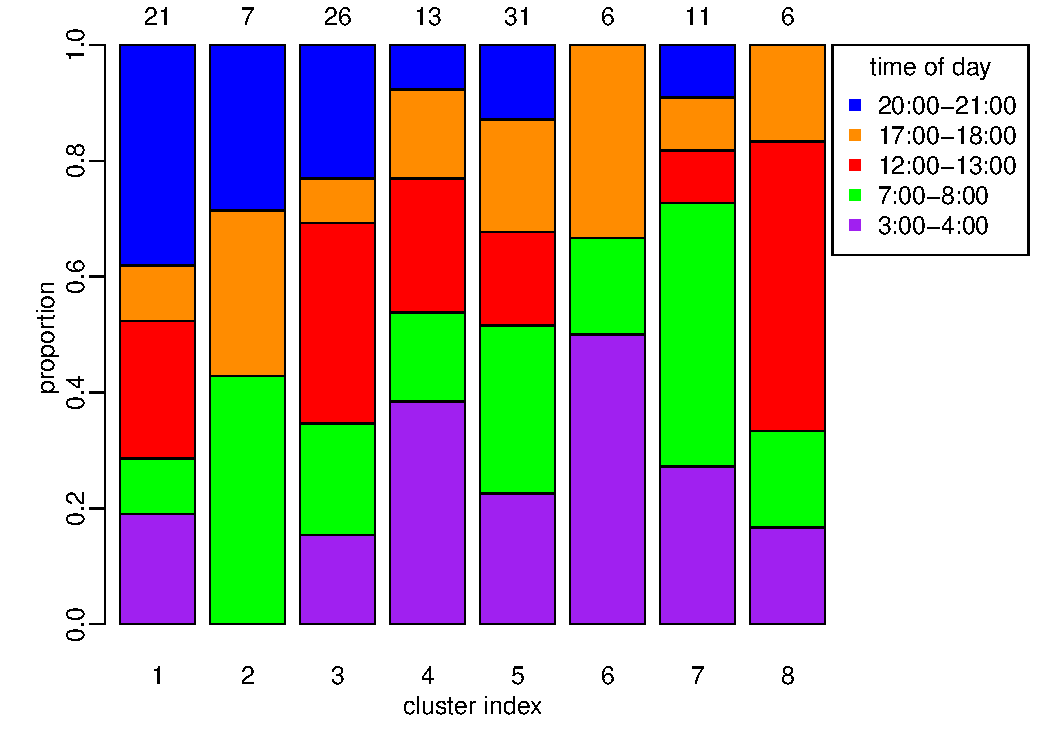
\includegraphics[height=0.42\hsize,width=0.53\hsize]{./figure/norm_comp-eucl-ward-8-timezone.pdf}
}~
\subfigure[曜日での分類(割合)]{
\hspace*{-0.6cm}
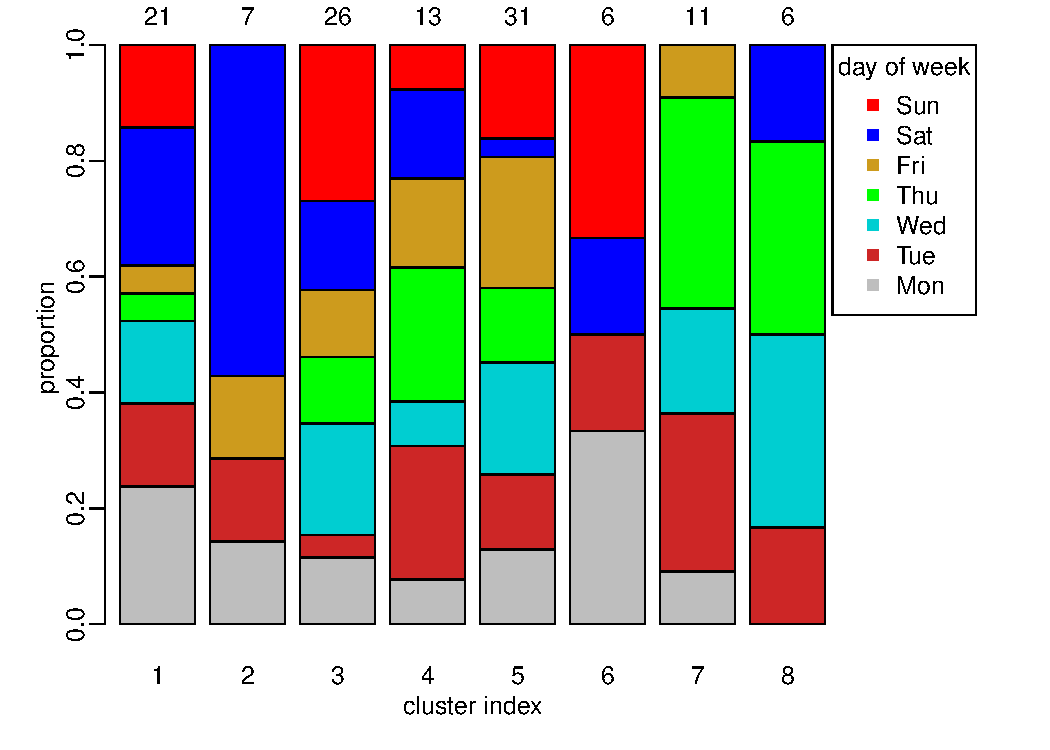
\includegraphics[height=0.42\hsize,width=0.53\hsize]{./figure/norm_comp-eucl-ward-8-day.pdf}
}\\
\subfigure[時間帯と曜日での分類(割合)]{
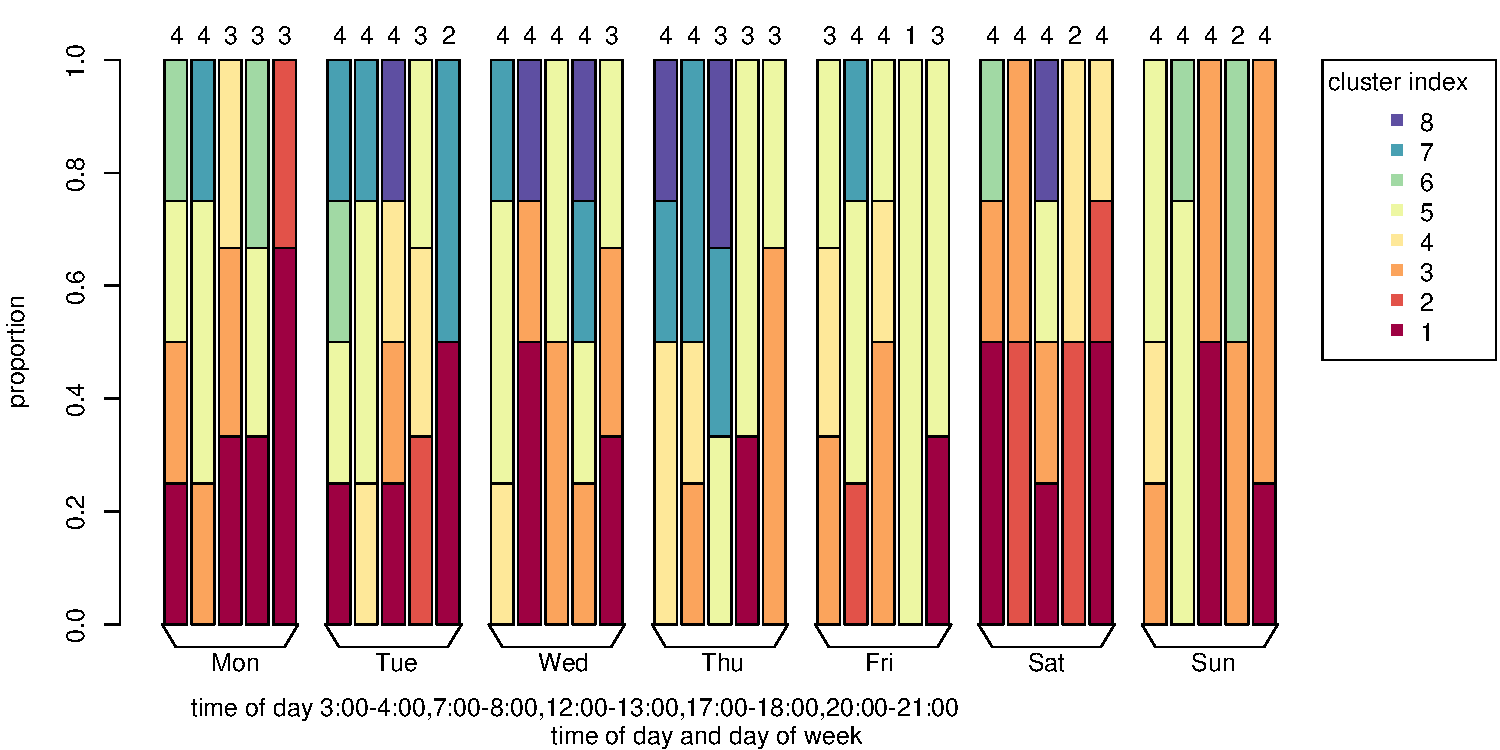
\includegraphics[height=0.42\hsize,width=\hsize]{./figure/norm_comp-eucl-ward-8-timezone-day.pdf}
}
\caption{実測値パラメータの主成分のクラスタリング結果}
\label{norm}
\end{center}
\end{figure}

\begin{figure}[tb]
\begin{center}
\subfigure[時間帯での分類(区間データ数)]{
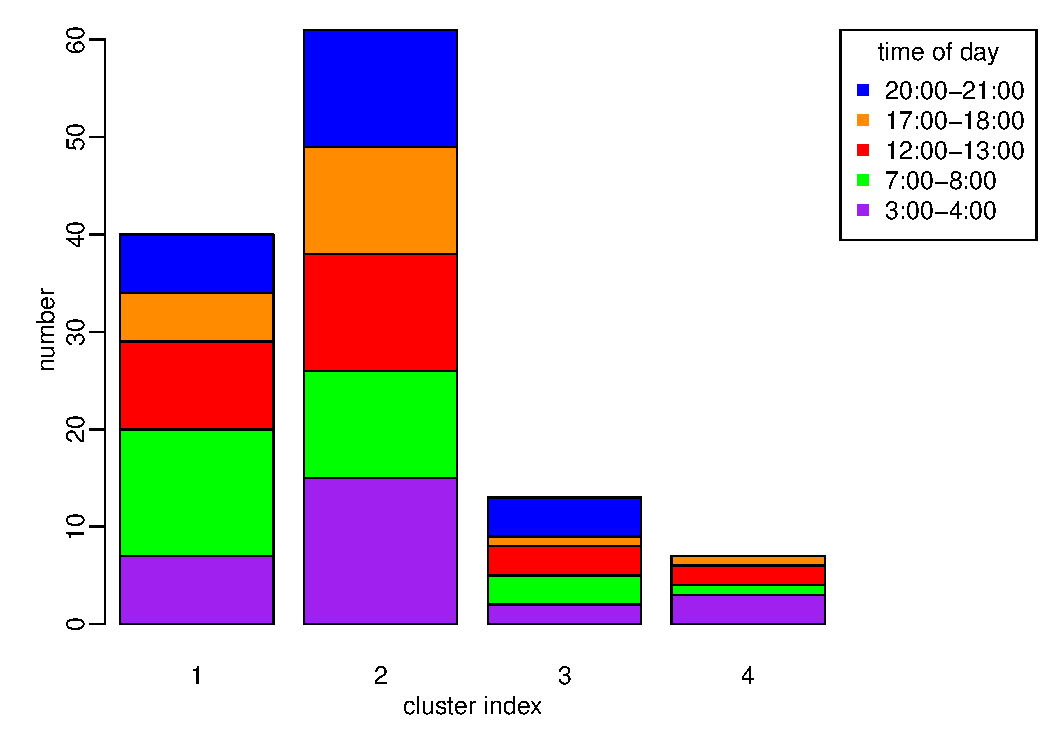
\includegraphics[height=0.42\hsize,width=0.53\hsize]{./figure/num-diff_comp-eucl-ward-4-timezone.pdf}
}~
\subfigure[曜日での分類(区間データ数)]{
\hspace*{-0.6cm}
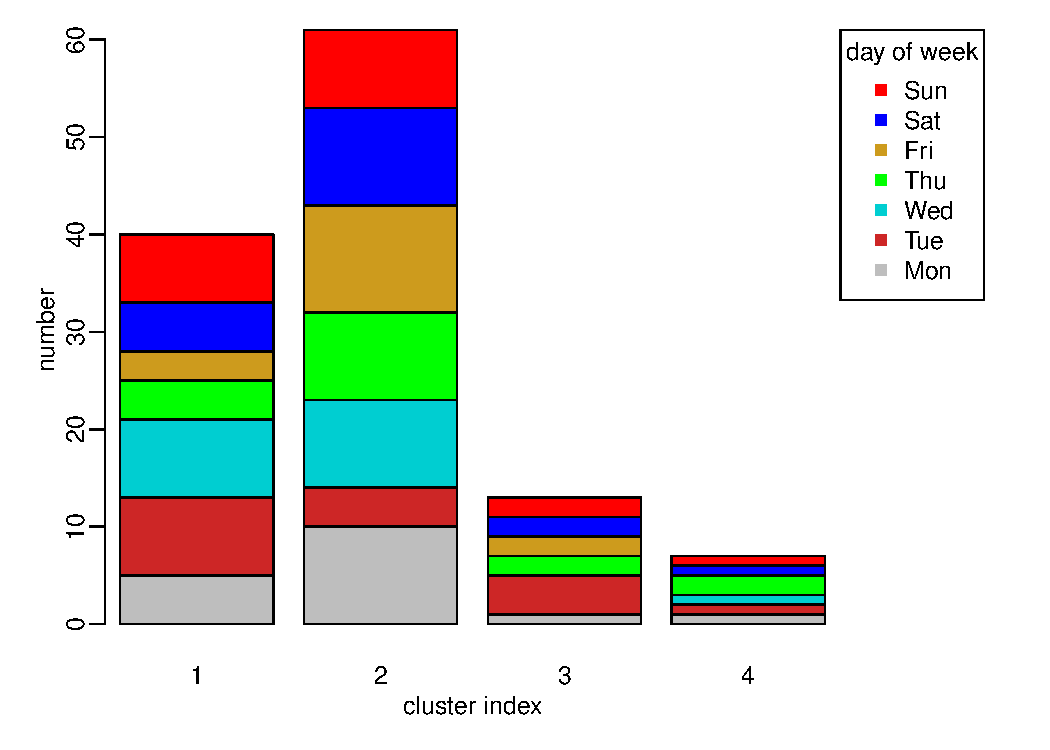
\includegraphics[height=0.42\hsize,width=0.53\hsize]{./figure/num-diff_comp-eucl-ward-4-day.pdf}
}\\
\subfigure[時間帯での分類(割合)]{
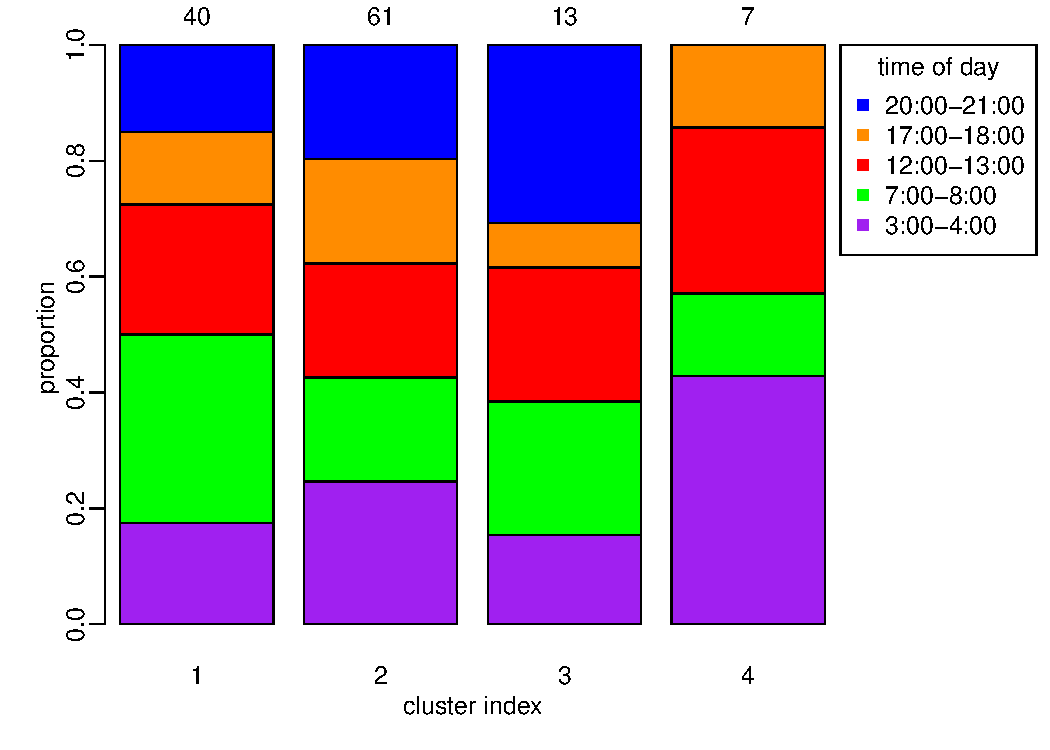
\includegraphics[height=0.42\hsize,width=0.53\hsize]{./figure/diff_comp-eucl-ward-4-timezone.pdf}
}~
\subfigure[曜日での分類(割合)]{
\hspace*{-0.6cm}
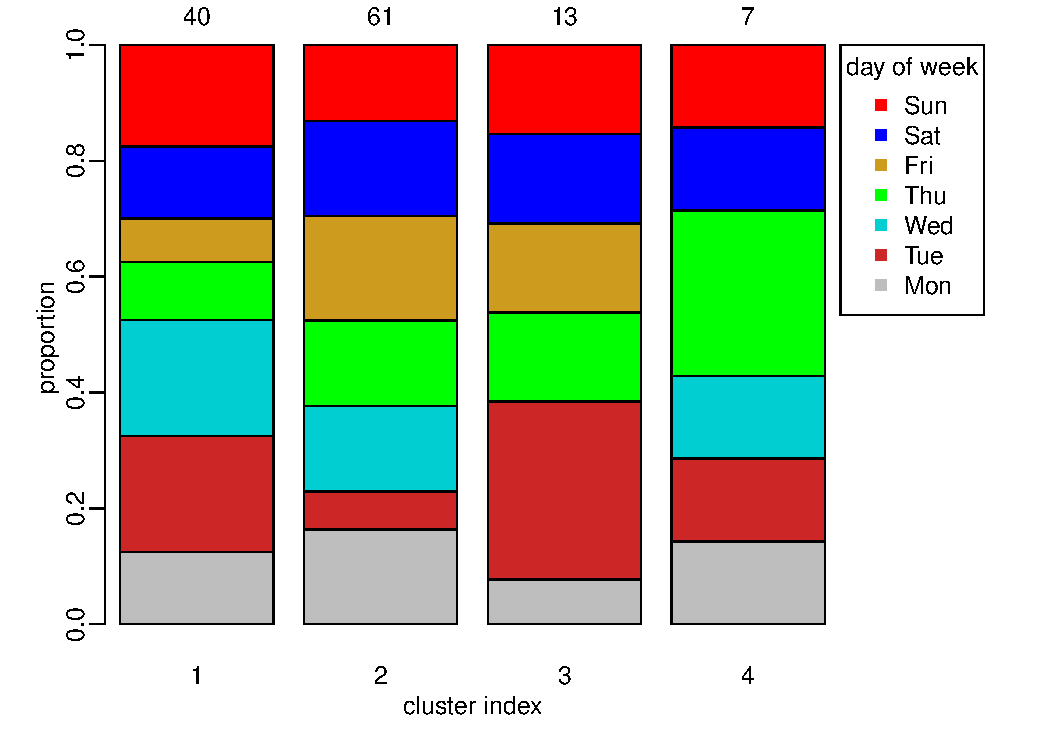
\includegraphics[height=0.42\hsize,width=0.53\hsize]{./figure/diff_comp-eucl-ward-4-day.pdf}
}\\
\subfigure[時間帯と曜日での分類(割合)]{
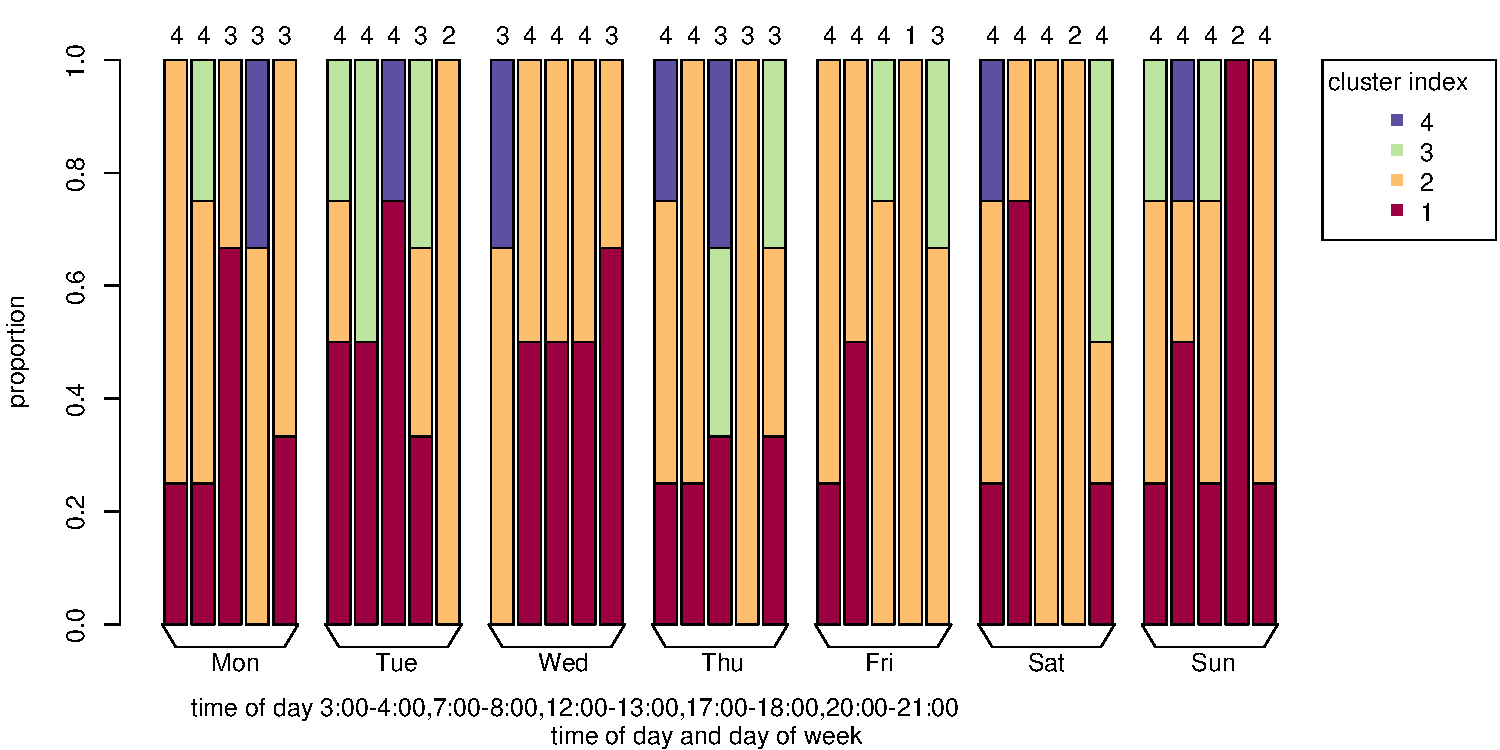
\includegraphics[height=0.42\hsize,width=\hsize]{./figure/diff_comp-eucl-ward-4-timezone-day.pdf}
}
\caption{変動値パラメータの主成分のクラスタリング結果}
\label{diff}
\end{center}
\end{figure}

図 \ref{norm}(a),(c) より,いずれのクラスタにおいてもすべての時間帯の区間データが一様に含まれているということはなく,属する区間データには時間帯による偏りがあることがわかる.
特に,図 \ref{norm}(e) より全ての曜日において 20 時台の区間データのうち少なくとも一つはクラスタ 1 に属していることがわかる.
20 時台は 21 時台のピークに向けて移動通信トラヒックが増加する時間帯であり(図 \ref{traffic})\cite{soumutrafficstatics},また,ネット利用の行為者率が最大になる時間帯である\cite{soumuwhitepaper}.
また,クラスタ 3 には同様に移動通信トラヒックが多い 12 時台の区間データが多く含まれている.
また,クラスタ 1 とクラスタ 3 には一日を通じてトラヒック量の多い土曜日と日曜日の区間データが多く含まれている.
また,平日のうち他の曜日と比べてトラヒックが多い月曜日の昼間の区間データはクラスタ 1 とクラスタ 3 に多く含まれている.
このことから,利用者の多い時間帯の応答遅延は似た傾向があり,そのうち,夜間の応答遅延の特徴を持つ区間データはクラスタ 1 に,昼間の応答遅延の特徴を持つ区間データはクラスタ 3 にそれぞれ分類されたものと考えられる.

クラスタ 5 とクラスタ 7 には 7 時台の区間データが多く属している.
また,クラスタ 5 には水曜日や金曜日の区間データが多く,一方でクラスタ 7 には土曜日と日曜日の区間データが含まれていない.
火曜日から金曜日に対して月曜日,土曜日,日曜日のトラヒックの変化は緩やかであることから,通信トラヒックの変化が激しい曜日の応答遅延は似たような傾向があり,それらがクラスタ 5 とクラスタ 7 に分類されたと考えられる.
また一方で,クラスタ 4 には,通信トラヒックが少ない 3 時台の区間データが比較的多く含まれ,一方で通信トラヒックが多い月曜日,土曜日,日曜日の区間データがあまりないことから,通信トラヒックが少ない場合の応答遅延には似た傾向があると考えられる.
クラスタ 2,6 および 8 については,それぞれ 7時台,3 時台,12 時台の区間データが占める割合が多いが,属する区間データの数が少ないため,特定の傾向を見いだすことができなかった.

\begin{figure}[tb]
\centering
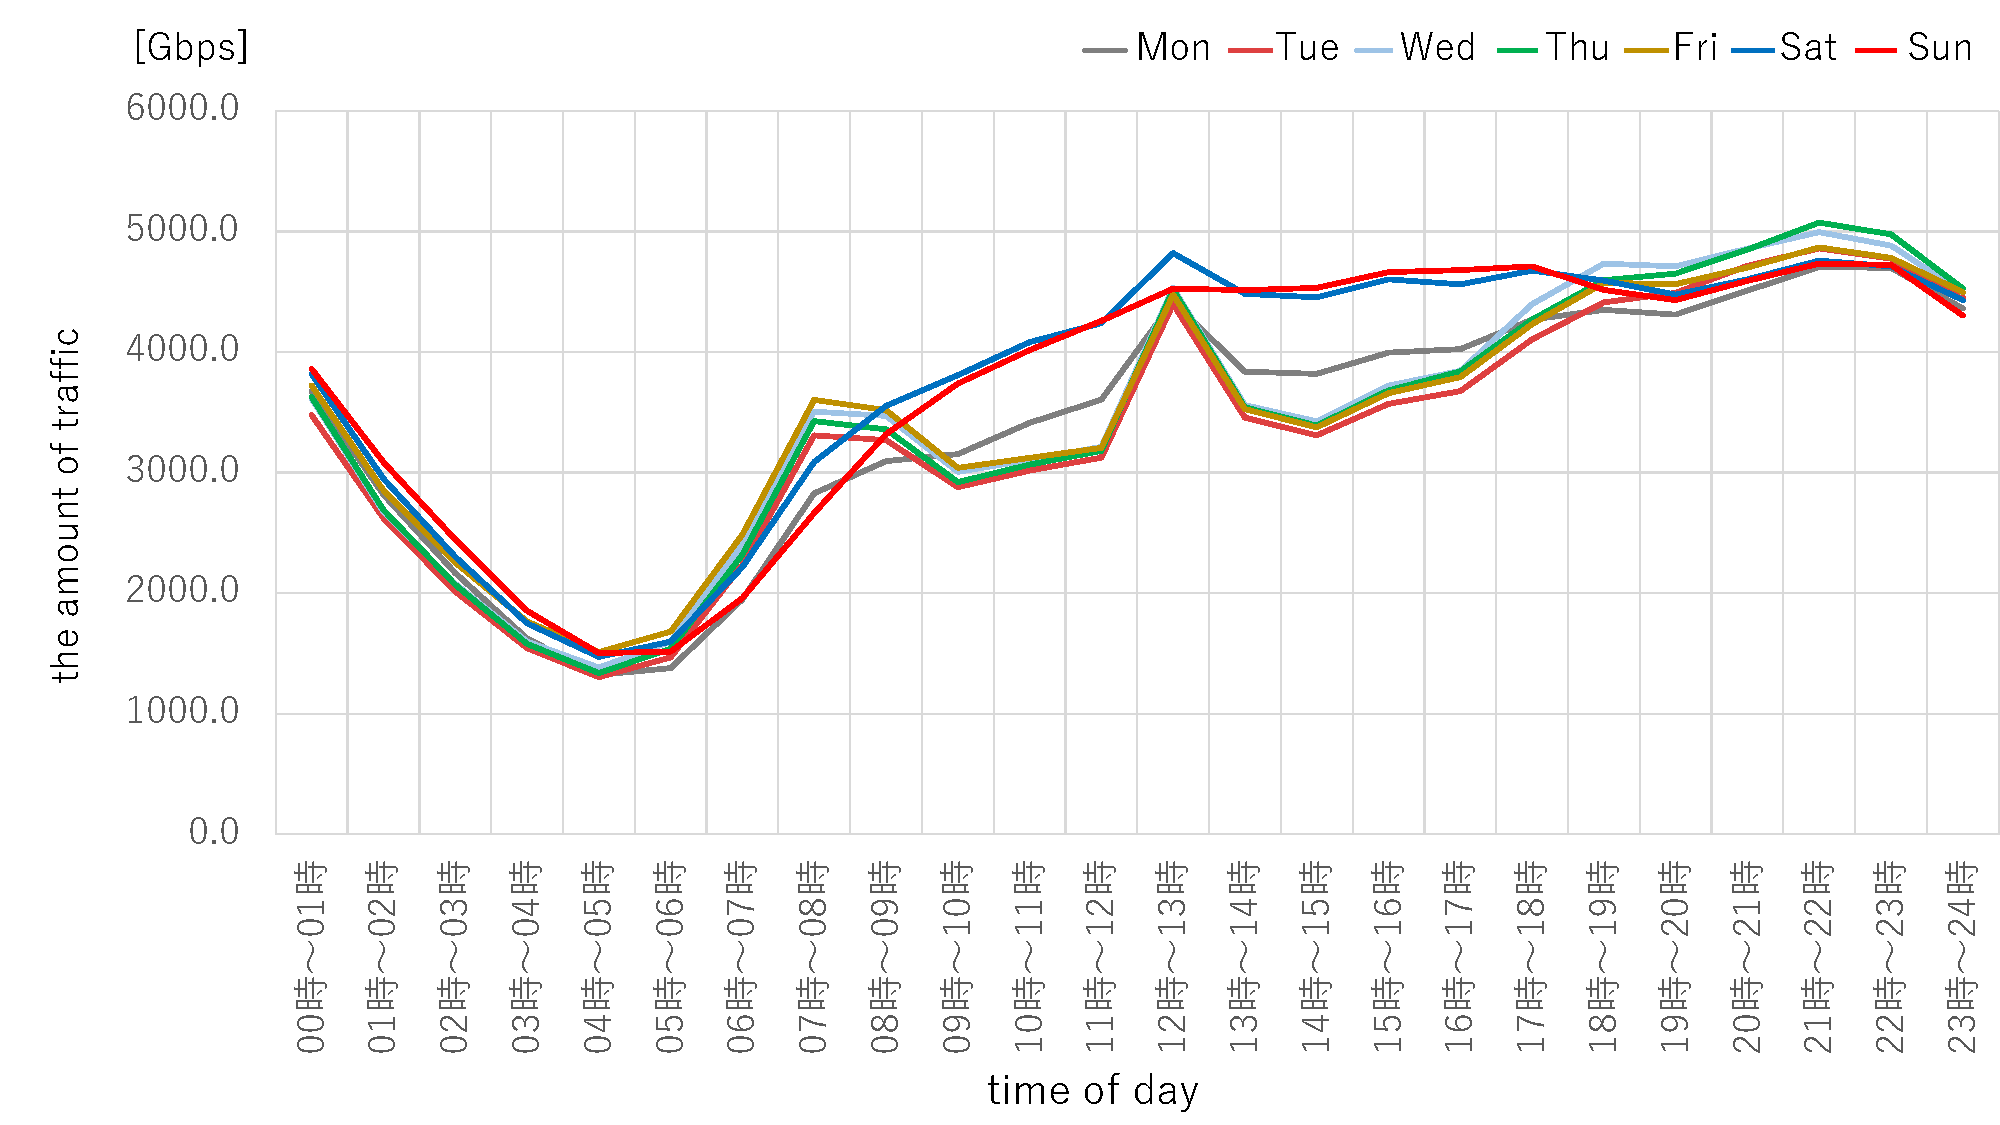
\includegraphics[height=0.55\hsize,width = \hsize]{./figure/traffic.pdf}
\caption{曜日ごとの時間帯と平均移動通信トラヒック量の関係}
\label{traffic}
\end{figure}

図 \ref{diff} より,変動値パラメータの主成分にもとづくクラスタリングでは,多くの区間データがクラスタ 1 と 2 に属していた.
また,クラスタ 1 と 2 との間には曜日や時間帯に応じた顕著な特徴を見出しにくい.
これは,変動値の系列が実測値の大きさによらず 0 msを中心に変化していることから,曜日や時間帯によらず似た傾向を示しやすいためであると考えられる.
一方で,クラスタ 3 とクラスタ 4 に属する区間データは通常時と異なる振る舞いを示していると考えられる.
なお,図 \ref{PseudoFwithMinPlot} に示すとおり,より細かな分類をするためにクラスタ数を増やすことは急激な Pseudo F with Min の低下を招くため望ましくない.

以上より,モデルパラメータの主成分によるクラスタリングにもとづいて異常検知を行う際には,実測値パラメータの主成分を対象とするのがよいと考えられる.
例えば,予備計測で生成されたクラスタのメドイドにより曜日や時間帯に応じたモデルパラメータの基準値を定め,そのもとで算出された推定値と運用環境における実測値が継続して大きく異なる場合に異常とする手法や,逐次的に時系列解析,クラスタリングを行い,区間データが通常と異なるクラスタに収容され続けた場合に異常とする手法が有効と考えられる.
\section{まとめと今後の課題}
本稿では,LTE ネットワークを通じたクラウドサーバとの応答遅延の計測を行い,産業用モニタリングシステムでの障害の検知,予測の実現に向けて,時系列モデリングやクラスタリングによってその特性分析に取り組んだ.
その結果,時系列モデリングの実測値では中期的な応答遅延変動を捉えることができ,また,変動値に対しては瞬時的な遅延の増加は追従できないもののおおむね精度良く時間変化を表せることを明らかにした.
また,実測値のモデルパラメータの主成分にもとづいてクラスタリングを行うことにより,応答遅延変動に曜日や時間帯によるモバイル通信トラヒックの変化に応じた傾向があることを示した.

今後の課題として,さらに長期間の計測,分析を行い,特に平時と異なるネットワーク利用が生じている状況での応答遅延の変動特性を明らかにすることが必要である.
その後,本稿で述べたような異常検知手法の設計を行い,その有効性を実データにもとづいて検証する.さらに,瞬時的な大きな応答遅延の発生頻度や発生間隔の分布などにもとづく異常の検知手法など,他の手法との組み合わせによる精度向上についても取り組む.

\bibliography{myrefs}
\bibliographystyle{sieicej}
\end{document}